\chapter{Test theories and automated test assembly models}
\label{ch:ATA}

Educational assessment addresses the problem of measuring the ability of students by modeling their responses to a test under a statistical perspective. Such test is a set of items selected from an item bank. A key aspect is that, as with any other measurement instrument, different measurements of the same ability should be comparable. In order to meet this requirement, tests should be standardized. A test is considered to be standardized when the test procedures are fixed in such a way that differences among testing conditions, times, and places, do not influence the scores \parencite{verschoor2007genetic}. The accuracy of measurement (test reliability), and the degree to which a test actually measures the ability it is supposed to measure (test validity) are fundamental issues in the development of standardized tests and in the production of a fair scoring system. As the test takers do not necessarily get the same test, it is fundamental that the conditions of reliability and validity are fulfilled through a systematic approach to test development, in which the assembly procedures play a very important role.

According to \textcite{downing2006twelve}, several phases in such an approach can be distinguished: project plan, content definition, test specifications, item development, item banking, pretesting, item bank calibration, test assembly, test production, test administration and reporting results. Several methods are used for test assembly nowadays. A common practice is selection by hand, usually after item analysis either based on classical test theory (CTT) or item response theory (IRT). However, in the last decades, modern technologies like sophisticated item banking systems and of open-source tools allowed the testing institutes to improve their assessment programs and test assembly process by substituting manual selection with automated test assembly (ATA). 

Moreover, the development of computer technologies enabled national test institutes to introduce the use of computers in educational testing. For example, in 2018 the Italian National Institute for the Educational Evaluation of Instruction and Training (INVALSI) adopted computer based testing (CBT) for grades 8 and 10 instead of the traditional paper and pencil (P\&P) testing. This chapter discusses the basics of ATA and the specific characteristics of the assembly procedures used in classical settings for automated test assembly. In Section \ref{sec:TestTheories}, the key theoretical issues of CTT and IRT, which represent the fundamentals of ATA, are briefly introduced. In Section \ref{sec:assembly-models}, the main features of the optimization models used in ATA are presented together with an indepth description of the Lagrange relaxation \parencite{fisher1981lagrangian} applied to the mentioned ATA models.



\section{Test Theories}
\label{sec:TestTheories}
In educational and psychological measurement, the process of test development follows specific steps \parencite[see e.g.,][]{downing2006twelve} which are guided from strong methodological test theories: classical test theory (CTT) and item response theory (IRT), respectively described in \textcite{lord1952theory} and \textcite{Hamb85,Hamb91}. The statistical framework of test theories was instead introduced in \textcite{lord1968statistical}. The major focus of CTT is on test-level information, while IRT primarily focuses on the item-level information. Especially IRT provides a good framework for automated test assembly methods because it is possible to compute the item Fisher information, a key object used to build optimal test in terms of accuracy of ability estimation.

\subsection{Classical test theory}\label{sec:ctt}

The fundamental assumption of CTT is that the true score of a person on a measurement, which is an unobservable variable, is the expected value of the observed raw score, i.e., the expected number-correct score over an infinite number of independent test administrations \parencite{novick1966axioms,lord1968statistical}. Given a person $n$, the observed score $X_n$ is defined as the sum of the true component and a random error component, as follows
\begin{equation}
X_n = \tau_n+\epsilon_n,
\end{equation}
where $\tau_n$ is the true score and $\epsilon_n$ is the normally distributed error term with expected value equal to zero and constant variance. Measurement errors are assumed to be uncorrelated over repeated administrations.

Within CTT, the test development process is based on checking the test validity and test reliability. In particular, the fundamental concept of reliability is concerned with the internal consistency of the test, i.e., the degree to which all item scores in a test correlate positively with one another. Given an item bank with items indexed by $i=1,\ldots,I$ and let $\mathcal{I}_t$ indicate the set of items taken in test $t$, the most popular index used to assess test reliability is the Cronbach's $\alpha$ \textcite{cronbach1951coefficient}, which is defined as
\begin{equation}
\alpha= \frac{|\mathcal{I}_t|}{1-|\mathcal{I}_t|}\left(1- \frac{\sum_{i \in \mathcal{I}_t}\sigma^2_i}{\sigma^2} \right),
\end{equation}

\noindent where $|\mathcal{I}_t|$ is the cardinality, i.e. the length of test $t$, $\sigma^2$ is the variance of the total test score and $\sigma^2_i$ is the variance of item $i$. The closer $\alpha$ to 1, the higher the test reliability. Unfortunately this function is non-linear with respect to the items and hence is not actively used in test assembly models which are usually linear. However, it can be employed to assess the consistency of the assembly results.

Two other item properties play an essential role in CTT: item difficulty and item discrimination. For dichotomously scored items, the difficulty of an item  $i$, in the item bank, is defined as the expected score given by a randomly selected examinee from the population of interest and is usually denoted by $\pi_i$ or \textit{p}-value $p_i$. The item discrimination is operationalized as the point-biserial correlation between the item score and the raw observed test score and denoted as $\rho_{it}$ for item $i$ and test $t$.

The main limitations of CTT are the test-dependent score, the existence of a single standard error of measurement for the population, and the focus at test level. These drawbacks are overcome by using IRT.

\subsection{Item response theory}\label{sec:irt}
An exhaustive introduction about IRT models can be found in \textcite{lord1968statistical, Hamb91}. Here, we are going to discuss IRT models with the only intention to supply their fundamental ideas and statistical notation needed to understand the subsequent sections. Very briefly, an IRT model expresses the relation between the observable variables (the item responses) and the unobservable, latent ability through a probabilistic model. It is assumed that the performance of an examinee can be explained through his/her latent ability(ies). The most popular IRT models are based on the unidimensionality assumption, i.e., the existence of a single latent ability independent between test-takers and the correct modeling of the phenomenon. However, multidimensional IRT models have been developed as well. A second assumption is local independence, which means that the item responses are statistically independent, conditional to the specification of the correct dimensionality (a single ability or a set of abilities).

A unidimensional IRT model for dichotomous items (e.g., correct-incorrect) expresses the probability of endorsing an item as a function of the underlying ability and a set of item parameters representing the item properties through a \textit{S}-shaped curve called item characteristic curve (ICC). This function is nonlinear in the ability, and it is monotone increasing because the idea behind these models is that the higher a person is located on the latent trait the higher is the probability she/he will give a correct answer. Different IRT models are characterized by the item response type, the number of item parameters, the latent ability structure, and the functional form.

The Rasch model, also known as the one-parameter logistic (1PL) model, has an ICC expressed by the following formula
\begin{equation}
P_i(\theta)=\frac{\exp(b_i+\theta)}{1+ \exp(b_i+\theta)},
\end{equation}

\noindent where $P_i(\theta)$ is the probability of a correct answer to item $i$ for an examinee of ability level $\theta \in (-\infty,\infty)$, and the parameter $b_i \in (-\infty,\infty) $ represents the easyness of the item $i$. We opted for the parametrization proper of the latent regression models because it simplifies the computations.

An example of ICCs for the Rasch model is shown in Figure \ref{fig:icc}. Note that the curves differ only by their location on the ability scale: the easiest item is C1 while the most difficult one is the C4. In fact, the Rasch model assumes that the easyness parameter is the only item characteristic that influences the examinee's performance.

\begin{figure}[h]
	\centering
	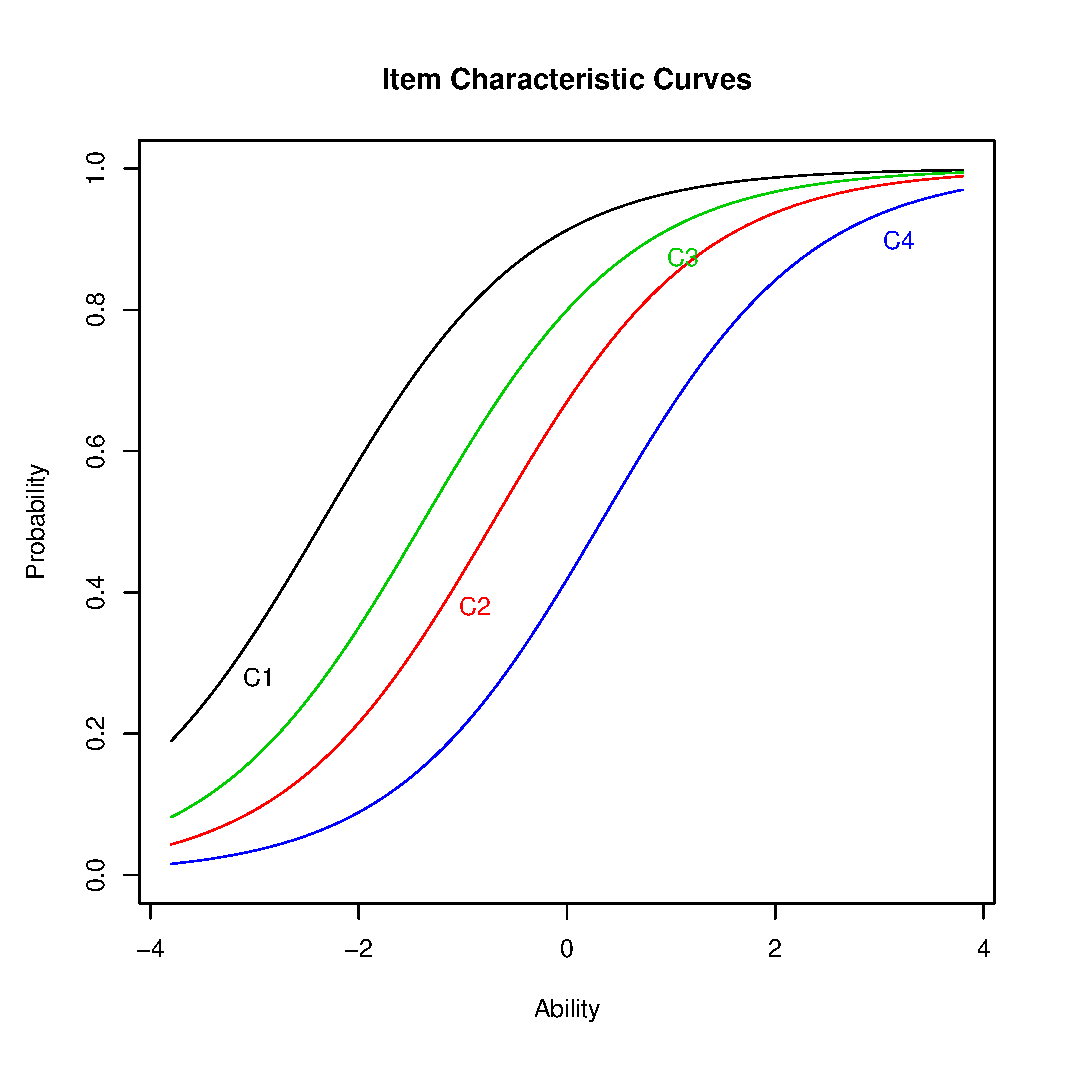
\includegraphics[scale=0.5]{icc.eps}
	\caption{ICCs of 4 items C1-C4 with different difficulties according to the Rasch model.}
	\label{fig:icc}
\end{figure}

IRT models allow the simultaneous estimation of the item parameters and the examinees' abilities. The \textit{calibration} process usually involves the estimation of item parameters from pre-test response data. The \textit{scoring} phase deals with the estimation of the ability scores of the candidates. Once the item parameters have been estimated, it is possible to understand how precise the test is at various ranges of the latent ability by using the test information function (TIF), which is defined as the sum of the item Fisher information for all the items in the test. In fact, under the maximum likelihood (ML) scoring, the Fisher information is asymptotically equal to the inverse of the variance of the ML estimator as follow,
\begin{equation}
I(\theta)=\frac{1}{\text{Var}(\hat{\theta}| \theta)}.
\end{equation}
The TIF has a very favourable property that is the additivity (and hence linearity) over the items of a test. Given a test with $k$ items, the TIF is equal to
\begin{equation}
I(\theta)=\sum_{i=1}^k{I_i(\theta)},
\end{equation}

\noindent where $I_i(\theta)$ is the item information function (IIF) for item $i$. Expressions for the IIFs can be easily derived within the framework of IRT. For example, for the Rasch model, the IIF of item $i$ is equal to
\begin{equation}\label{eq:infofun2pl}
I_i(\theta)=P_i(\theta)(1-P_i(\theta))=\frac{\exp^{(b_i+\theta)}}{[1+\exp^{(b_i+\theta)}]^2}.
\end{equation}
An example of IIFs for the Rasch model is shown in Figure \ref{fig:iif}. The items are maximally informative (information equal to 0.25) at the ability level corresponding to the easyness parameter.

\begin{figure}[H]
	\centering
	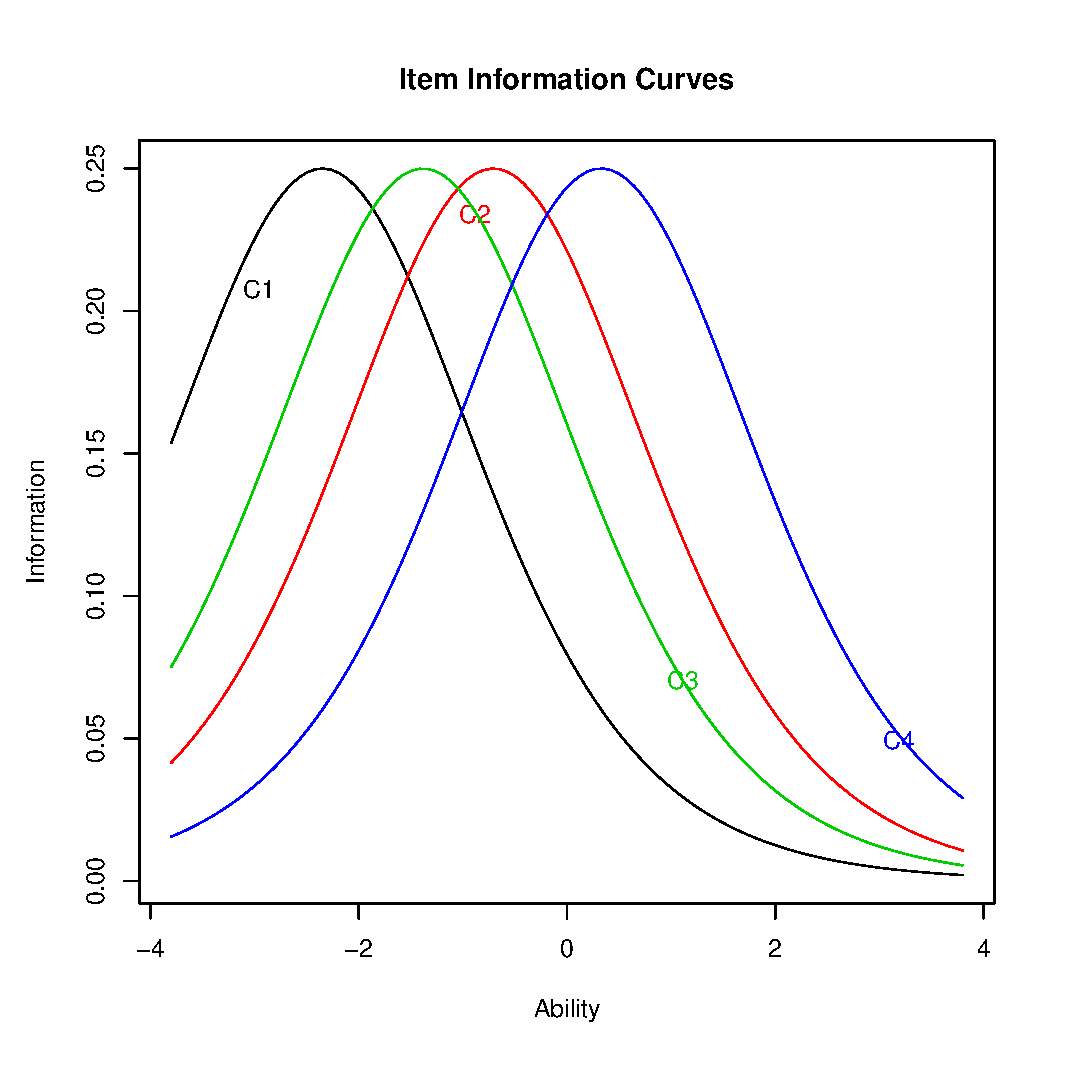
\includegraphics[scale=0.5]{iif.eps}
	\caption{IIFs of 4 items C1-C4 according to the Rasch model.}
	\label{fig:iif}
\end{figure}

Figure \ref{fig:tif} shows a test information function for a test with 10 items. The Fisher information function is a critical element in test assembly because of its linearity and its easy interpretation. Tests can be assembled merely through the selection of appropriate items out of an item bank, one way to do so is to use mathematical programming techniques like 0-1 linear programming (LP) or mixed integer programming (MIP) models. Using these approaches the tests can be built by, for instance, maximizing the TIF at predefined $\theta$ points (MAXIMIN in this dissertation), or matching it with known optimal values (MINIMAX) with linear restrictions on the values of items properties.

\begin{figure}[H]
	\centering
	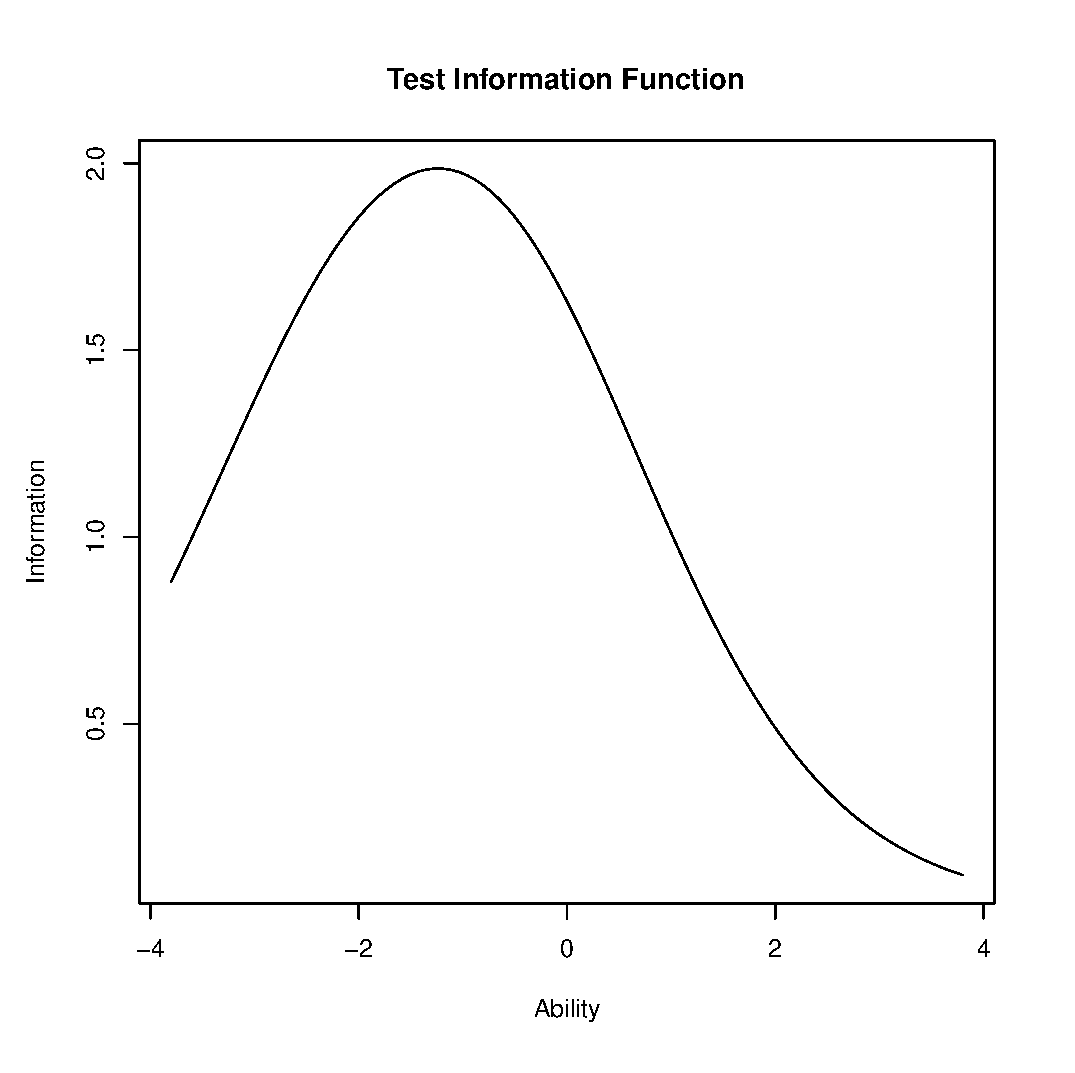
\includegraphics[scale=0.5]{tif.eps}
	\caption{An example of test information function (TIF).}
	\label{fig:tif}
\end{figure}

The two-parameter logistic (2PL) model \parencite{birnbaum1958} is a generalization of the Rasch model. Like the Rasch model, the 2PL assumes that the probability of a correct response to an item $i$ depends on the difference between the respondent’s trait level $\theta$ and the easiness of the item $b_i$. Also, the 2PL postulates that for every item, the association between this difference and the response probability depends on an additional item discrimination parameter: $a_i$. 
The ICC of the 2PL IRT model is given by:
\begin{equation}
P_i(\theta)=\frac{\exp(b_i+a_i\theta)}{1+ \exp(b_i+a_i\theta)}.
\end{equation}

The probability of a positive response (e.g., solving an item correctly) is strictly monotonic, increasing in $\theta$ and $b_i$. The item discrimination parameter characterizes how fast the probability of endorsing the item approaches $1.00$ with increasing trait level when compared to other items. In other words, the model accounts for the possibility that responses to different items are not equally strongly related to the latent trait. The discrimination parameter describes how well a particular item discriminates between examinees with different trait levels compared to other items on the test. 

We decided to focus on the 2PL model because it is widely used in practical applications, \textcite{desimone2015item}

\section{Automated test assembly}\label{sec:ata}

In the late 1970s, the transition from paper-and-pencil to computer-based tests has begun in the United States, increasing the efficiency and the accuracy of the assessment tools. First of all, the administration of tests by computers streamlined the process of data collection and recording, allowing to have scores immediately available
and free of data entry errors. Secondly, skills and variables that could not be assessed or measured by paper-and-pencil tests like higher-level thinking skills, complex problem-solving and response times now are quickly recorded and evaluated thanks to the computers. The growing number of credentialing exams for allowing the practice of a profession, admission tests for granting the access to the universities and standardized national tests for comparing abilities among different settings increased the importance of the use of test scores and hence the content and statistical features of the tests became crucial for the test validity and reliability.

ATA was born in this framework where fulfilling several specific requirements on the tests such as reducing the length of the test, maximizing the precision of the ability estimates, building tests with the same difficulty level and moreover, were needed. In practice by ATA models, a test developer can impose any content and statistical criteria, from here called constraints, by specifying them in the form of linear (in)equalities. Also, a test developer could choose an objective function to serve as the goal for test assembly. Therefore the computer can find a set of test items that optimally meet these specifications. It is clear that test assembly is at the heart of the test development process but the automatically produced test is only a first draft of tests that could then be reviewed and re-examined by committees.

At the time when the test is assembled, the input is required from
three other processes: test specification, item construction and test data
analysis. A good test needs good specifications, good items and good data.

\subsection{The item bank}\label{sec:the-item-bank}

Once the calibration has been done, the items and their estimated and structural properties are stored in the \emph{item bank} (or item pool). Afterward, we can move on to the test assembly procedure in which the items will be selected depending on those distinctive characteristics.

Table \ref{tab:bankex} shows an example of the structure of an item bank with $I$ items, where the items are displayed by row while in the columns we find the items features, from left to right: the identifier (\textsl{ID}), the IRT difficulty parameter ($b$) together with its standard error ($b_{se}$), CTT difficulty (\textsl{p-value}), content attributes (\textsl{TYPE}, \textsl{PROCESS}, \textsl{DOMAIN}), and relational attributes that specifies if the item belongs or not to a specific set (\textsl{FRIEND SET 1}, \textsl{FRIEND SET 2}, \textsl{ENEMY SET 1}, \textsl{ENEMY SET 2}).

Examinees can get different sets of items because, thanks to the calibration via IRT, the items are set on the same scale and the examinees' scores can be compared.

\subsection{Types of assembly models}\label{sec:assembly-models}

Given an item bank containing a sufficient number of calibrated items, is it possible to assemble one or more test forms which features can be similar or diverge. When we need to assemble only one test form we are speaking about \emph{single tests assembly} models while if the tests are more than one the models are for \emph{multiple tests assembly}, in particular, if the obtained ones are similar under their psychometric characteristics they are called \emph{parallel} \footnote{Other details in Section \ref{sec:multiple-test-assembly}.}.
In this work, we will focus on the latter category of automated test assembly models.

To solve this type of problems in the last decades three modes of automated test assembly became prevalent: sequential, simultaneous single or multiple test assembly and adaptive tests.
By the first two, test forms are entirely built before the administration of the test while in the adaptive framework, each test form is assembled during the testing procedure.

\subsubsection{Sequential test assembly}

The straightforward technique for assembling single or multiple test forms is to populate the forms with items in a sequential way. This is being done by selecting items or groups of items and removing them from the pool; then the model is adapted to the new pool to try to fit the next form. In the case of assembling parallel forms, this method has two serious disadvantages. First, if the forms are assembled one after the other, the value of the objective function for the solution of the model tends to decrease due to the fact that the items with the best values will be selected first. As a consequence, the forms will not be parallel. The second disadvantage of
this approach is the possible infeasibility of later models in the sequence. On the other hand, by this type of model, an extensive range of functions can be optimized, e.g., the linear structure of the problem can be relaxed. Most of these problems nowadays are solved using ad hoc greedy and heuristic techniques.

\subsubsection{Simultaneous test assembly}

In the sequential approach, an incremental number of different models must be optimized in order to obtained multiple forms causing the disadvantages cited in the last paragraph. Those can be overcome by applying simultaneous test assembly models in which the solution, and hence, the test forms, is obtained by solving only one model. They are usually represented by 0-1 integer programming problems and solved by linear programming techniques. The model can be reformulated as a mathematical optimization problem using decision variables. Decision variables are variables defined such that the solution of the optimization problem (i.e., the set of values for which the objective function is optimal and all constraints are satisfied) identifies the best decision that can be made. The decision variables $\{x\}_{it}$ are binary (0-1) since they represent the inclusion (1) or exclusion (0) of the item $i$ in the test $t$. In the last decades, the algorithms needed to solve such optimization problems were improved, and nowadays, powerful implementations of them are available as commercial or open-source software.

\subsubsection{Adaptive tests}

In the adaptive approach, one item is optimally picked from the pool at a time. The person's ability estimate is updated during the test, and each next item is chosen to be maximally informative at the last ability update. The test is then tailored to the candidate. Because the ability estimates converge to the person's true ability level, item selection improves during the test and the ideal test with maximum information at the person's true ability level is approached. In the early 1990s computerized adaptive testing (CAT) was implemented in large-scale testing programs, and nowadays large numbers of subjects are tested worldwide using this type of test assembly. One of the most important benefits of this method is that it's more efficient, i.e., it is possible to get more precise ability estimates with fewer items than the previous standard approaches, but at the cost that it's quite impossible to ensure the congruence between tests since all the test takers will get a different set of items from the pool.

The description of different approaches to assemble tests is not finished here. Because of its advantages, the approach dealt with in this report is the simultaneous tests assembly mode.
In Section \ref{sec:single-test-assembly} and Section \ref{sec:multiple-test-assembly} we introduce the reader to the standard test assembly models used to build first, a single test form and secondly, as a generalization, multiple test forms.

\subsection{Single test form assembly}\label{sec:single-test-assembly}

As already discussed, a new testing program starts with formulating the set of specifications for the test to be met, that here we call \emph{desiderata}. Sometimes they are verbally expressed as a set of learning objectives or a list of dos and don'ts for the test developer, but they can also be well-structured in tables specifying how many items should have certain content or even better the distribution of items according to their specific characteristics.

Once the desiderata have been collected, they must be translated into a standardized language used in test assembly problems. The standard form in these problems is an \textit{objective function} to be optimized subject to several \textit{constraints}, where the latter define a possibly feasible set of tests for a given item bank, and the former expresses our preferences for the tests in this feasible set. If the specifications have been formulated in a simple, concise, but complete way, it is possible to determine whether they are objectives or constraints. These requirements are crucial for a correct translation of the desiderata into the standard language for test assembly problems: disambiguations and possible complications may arise in test design if these principles are not satisfied. An example of verbal test specifications is described in the Table \ref{tab:exspec}, which is partially extracted from \textcite{VDL2005}.
\begin{table}[H]
	\centering
	\begin{tabular}{|ll|}
		\hline & \\
		1. & Average \textit{p}-value of each test between .40 and .60 \\
		2. & Number of items on applications equal to 24 \\
		3. & Reliability of the test should be as high as possible \\
		4. & Items 73 and 100 never in the same test \\
		5. & Test information function as close as possible to the target \\
		6. & Items 33, 45 and 12 must be in the same test \\
		& \\
		\hline
	\end{tabular}
	\caption{Examples of desiderata.}\label{tab:exspec}
\end{table}

The specifications in Table \ref{tab:exspec} may represent either objectives or constraints; for example, points 1,2,4 are constraints while 3 and 5 are objectives. It is clear now that the objectives involve maximize or minimize some attributes, such as minimize the gap between the test information function at some $\theta$ point to its target (5) or maximize the reliability of the test (3) and on the other hand constraints impose a bound on an attribute of the test or of the items, such as limiting the difficulty of the test (1), fixing the number of items having specific characteristics (2) or considering enemy sets (4) or also item (friend) sets (6). An exhaustive classification of specifications together with examples of not well-expressed desiderata can be found at pages 34-39 of \textcite{VDL2005}.

\subsubsection{Standard form of a test assembly problem}

If a set of desiderata is well specified they can always be represented in the standard form of Table \ref{tab:stform}.
\begin{table}[H]
	\centering
	\begin{tabular}{|ll|}
		\hline    & \\
		optimize & \textit{Objective function} \\
		subject to & \\
		& \textit{Constraint 1} \\
		& \textit{Constraint 2} \\
		& $\vdots$ \\
		& \textit{Constraint N} \\
		& \\
		\hline
	\end{tabular}
	\caption{Standard form of a test assembly problem.}\label{tab:stform}
\end{table}

Only one objective can be optimized at a time; if we have more than one function to optimize some tricks can be applied to transform the objectives into constraints. On the other hand, there is no upper limit for the number of constraints, provided our solver can handle the problem. If at least one combination of items that meets all the constraints do exist, then the set of these combinations is called \emph{feasible set}; if this set is empty, we say that the model in \emph{infeasible}. The subset of tests in the feasible set that optimizes the objective function is called \emph{optimal feasible solution}.

\subsubsection{Decision variables}

Modeling a test assembly problem does not imply only defining objectives and constraints, but we also need the so-called \emph{decision variables} which represent the possible combination of items that compose the test form in a mathematical formulation. If we need to assemble a single test from a pool of $I$ items, we can choose as decision variables $I$ binary variables in the form:
\begin{equation*}\label{eq:optvar}
x_{i}=
\begin{cases}
1 & \mbox{if item }i \mbox{ is in the test},\\
0 & \mbox{otherwise}.
\end{cases}
\end{equation*}
We can also write the $x_i$ in an algebraic way using the vector $x$ of length $I$. Therefore we have $2^I$ possible combinations of values the vector $x$ can take. These combinations decrease in number if we add constraints to the model. In the following Section, we will also use nonbinary variables like integer o continuous, which are often useful to reduce the number of objectives in the problem. Once the decision variables have been identified, the process of modeling a test assembly problem goes through the steps of modeling the constraints and objectives and solving the model looking for an optimal solution.
In the following Section, we will present the basic formulations for some common types of constraints and objectives. The last step consists of solving the model by using a computer program which implements some mathematical or numerical algorithms.

\subsubsection{The model for assembling a single test}
The models presented in this Section are based mainly on item response theory attributes and we will make an almost exhaustive list of categories of constraints that can be added to a model for single test assembly together with possible objective functions.

The standard model for the assembly of a single test with a generic quantitative objective from a pool of $I$ items indexed by $i=1,\ldots,I$ is
\begin{subequations}\label{eq:singClassTest}
	\begin{equation}\label{eq:Sobj}
	\mbox{optimize } {\sum_{i=1}^I q_i x_{i}} \quad \mbox{(objective)}
	\end{equation}
	subject to    
	\begin{alignat}{4}
	\label{eq:Scat}
	&n^{\min}_{c} \ &\le & \sum_{i \in V_c} x_i &\le \ & n^{\max}_{c}, \ & \forall c \quad & \mbox{(categorical constraints)}\\
	\label{eq:Squan}
	&b^{\min}_{q} \ &\le & \sum_{i=1}^I q_i x_i &\le \ & b^{\max}_{q}, \ &              \quad & \mbox{(quantitative constraints)}\\
	\label{eq:Slen}
	&n^{\min}      \ &\leq & \sum_{i=1}^I x_i &\le \ & n^{\max},      \ &             \quad & \mbox{(test length)}\\
	\label{eq:Sene}
	&    \ & & \sum_{i \in V_e} x_i&\le \ & 1,              \ & \forall e \quad & \mbox{(enemy sets)}.
	\end{alignat}
	Then, the definition of variables
	\begin{equation*}
	x_i \in \{0,1\}, \ \forall i \quad \mbox{(decision variables)}.
	\end{equation*}
\end{subequations}

\noindent In case the sums in the constraints are bounded only on one side, we only need one of the two inequalities.

For a qualitative variable, we use $V_c$ to represent the set of indices of the variable of the items in subset $c$. Allowing the test to have several items with specific qualitative attribute represented by $V_c$ between $n^{\min}_{c}$ and $n^{\max}_{c}$ means adding a \textit{categorical constraint} to the model. An example of a categorical constraint is ``the test must contain at least 10 items in problem-solving'', where the set of items in the pool that has the attribute ``problem solving'' is represented by $V_\text{problem solving}$ and $n^{\max}_\text{problem solving}=10$.

On the other hand, if we want to bound the value of a quantitative variable (i.e. that can take numerical values) addressed by the symbol $q$ between the values $b^{\min}_{q}$ and     $b^{\max}_{q}$ we are constraining the model adding a \textit{quantitative constraint} where $q_i$ is the value that the item $i$ takes for that variable. Suppose we want to assemble a test with the following criterion ``the maximum of words must be 300'', $q_i$ will serve as the number of words displayed by the item $i$ and $b^{\max}_{q}=300$.

The interpretation of the \textit{test length} constraint is straightforward as it is a special case of a quantitative constraint where $q_i=1$ for each $i=1,\ldots,I$.
If there are \textit{enemy sets} in our pool then the items in one of these sets, called $V_e$, cannot be picked together, e.g., the desideratum ``items 23 and 46 cannot be in the same test'' means that items 23 and 46 are enemies and both are in the enemy set $V_e$. Therefore the sum of the corresponding decision variables $x_{23}$ and $x_{46}$ cannot be more than 1.

\subsubsection{Item sets}\label{sec:item-sets}
Tests with sets of items organized around common stimuli (known as item sets or friend sets) are popular because of the efficiency of their format. By combining more than one item with the same stimulus, we can ask questions using more complex stimuli, such as reading passages, descriptions of cases, or problems with data in a set of tables or graphs, without having to sacrifice too many items for the test to meet the time limit. However, the presence of such sets in the item pool complicates the process of assembling the test. In particular, if the items are grouped in $S$ item sets or stimuli indexed by $s$, there are three ways to deal with this problem \parencite[see][]{VDL2005}.

\begin{itemize}
	\item The \textit{power set method} that consists in summarizing all the quantitative and qualitative attributes by summing or averaging them taking as groups the item sets; if we only need to constraint the test at the set/stimuli level the problem decreases in size since you don't have $I$ decision variables anymore but just $S$. This method is not efficient if you have variables that cannot be summarized, such as standard errors and if you want to keep some constraints at item level since you need to consider again the original decision variables $x_i$ increasing the size of the model.
	\item The \textit{pivot-item method} in which each set is represented by a pivot decision variable $x_{i^*_s}$ arbitrarily chosen. Therefore, we can use the variable for a pivot item as a carrier of the attributes of both its stimulus and item set, and we can drop the stimulus variables in the model.
	\item The \textit{two-stage method} that is a sequential approach with two phases, in the first, stimuli are selected and secondly, the model chooses the items with those stimuli.
	
\end{itemize}

Given the earlier warnings about sequential approaches we do not suggest the two-stage method and since all the variables in our item bank are summarizable (e.g., the item information function is additive, so it is possible to sum it for all the items in the stimulus) we prefer to adopt the power set method which helps to decrease the size of the problem.
The power-set formulation needs a phase of preprocessing of the item bank. Instead, for the formal representation of the model, we refer to \textcite[Section 7.2, ][]{VDL2005}.

\subsubsection{Single test MINIMAX}\label{sec:single-test-minimax}
Once we defined all the constraints and checked that the model is feasible, we need to choose an objective to optimize. A first option is to choose absolute targets for the TIF, targets are the values that a goal TIF assumes on a fixed number of $\theta$ points along the $\theta$ scale, these values must be chosen by test specialists who knows how much precision is required to estimate the abilities of the students at each ability level. That is the reason why absolute targets are used almost exclusively when tests are assembled to be parallel with respect to a known reference test. Formalizing this requirement in the standard form of test assembly models will produce a multi-objective test assembly problem that must be reformulated using the MINIMAX approach explained below.

In particular with the following addition to the model \eqref{eq:singClassTest} we ask that the TIF of the resulting test approximates with minimum negative and positive deviations (i.e., with the highest precision) the chosen goal TIF in a finite set of points $V$ on the $\theta$ scale, which we denote as $T_{k}$ with $k \in V$:
\begin{subequations}[intermezzo]
	\begin{equation}
	\mbox{minimize } \ y \quad \mbox{(objective)}
	\end{equation}
	subject to
	\begin{alignat}{2}
	\label{eq:SMINIMAX1}
	\sum_{i=1}^I I_i(\theta_{k}) x_{i} & \le T_{k}+ y, &\ \forall k \in V \\
	\label{eq:SMINIMAX2}
	\sum_{i=1}^I I_i(\theta_{k}) x_{i} & \ge T_{k}- y, &\ \forall k \in V
	\end{alignat}
	\begin{equation*}
	y \ge 0.
	\end{equation*}
	\label{eq:SMINIMAX}
\end{subequations}

More $\theta$ points are chosen more the TIF of the assembled test will meet the desired one, usually 3-5 points are enough to have a good approximation.

\subsubsection{Single test MAXIMIN}\label{sec:single-test-maximin}
If a reference test or absolute targets are not available, an alternative approach is trying to achieve the best predictive validity for the test, that is maximizing the TIF in some chosen theta points. This goal can be met not only setting the location of the peaks of the TIF but also defining its shape in the entire $\theta$ scale, which is to say imposing relative targets.

So, denoting with $R_k$ the relative targets for each $\theta_k$ with $k$ in the chosen set $V$ of ability points in which we want to control the shape of the TIF, we must fix one of the relative targets to a value (e.g. $R_1=1$) and all the other target values must be adjusted correspondingly trying to reproduce the wanted shape. Like the absolute target model, this method leads to have more than one objective function and, also in this case, it is possible to rely on a simplifying approach called MAXIMIN. The model can be formalized as follows:
\begin{subequations}\label{eq:MAXIMIN}
	\begin{equation}
	\mbox{maximize } \ y \quad \mbox{(objective)}
	\end{equation}
	subject to
	\begin{equation}\label{eq:SMAXIMIN1}
	\sum_{i=1}^I I_i(\theta_{k}) x_{i} \ge yR_{k}, \ \forall t,k \in V
	\end{equation}
	\begin{equation*}
	y \ge 0.
	\end{equation*}
	\label{eq:SMAXIMIN}
\end{subequations}

\noindent Also here, the practice suggests that the minimum number of $\theta$ points in which maximize the TIF must be 3 or 5.

\subsection{Multiple simultaneous test assembly}\label{sec:multiple-test-assembly}
%\par The models presented in the previous chapters are to assemble single test, however

In order to discourage the phenomenon of cheating, it is necessary to administer different items to the test takers. This can be achieved building more than one test form that contains different items preserving some overall mutual psychometric features, such as the same test difficulty or same content structure such as the same percentage of items of a certain stimulus. These tests are called \emph{parallel} (or interchangeable) and the procedure aimed to perform this task is called ``multiple test assembly''. In particular, test forms are defined to be \emph{weakly parallel} if their information functions are identical \textcite{same77}. On the other hand, test forms are \emph{strongly parallel} if they have the same test length and the exact test characteristic function \textcite{Lord80}.

As a consequence, we typically have problems with more objectives than those presented in Section \ref{sec:single-test-assembly} for a single test assembly. For example, if we assemble $T$ tests and each test has to meet a target for its information function at $K$ ability points (the same points for each test $t$, with $t=1,\dots, T$), the problem has at least $T \times K$ objectives. However, these sizeable multi-objective test assembly problems can be solved using a direct generalization of the approaches for single test assembly. In the following, we will present a general model for simultaneous assembly of a set of tests (that is, as a solution to a single model) that produces an optimal solution.
This type of assembly requires a reorganization of the problem using a different version of the decision variables. These variables have double indices\footnote{We use a matrix representation only for a better visual idea, actually they are still vectors but of bigger size.}, one for the items in the pool and the other for the test forms. For the current problem, the variables become
\begin{equation*}\label{eq:MDV}
x_{it} =
\begin{cases}
1, & \mbox{if item } i \mbox{ is assigned to test }t\\
0, & \mbox{otherwise}
\end{cases}
\end{equation*}

\noindent for all $i$ and $t$. As before, we need to complement these variables with a set of constraints that keep their values consistent. The adapted single test assembly model is presented here followed by constraints that arise only in the case of multiple test assembly.

\subsubsection{The model for assembling multiple tests}
Using the above decision variables, any model for a single test can be reformulated as a model for multiple tests. To illustrate this statement, we reformulate the standard model for a single test in \eqref{eq:Sobj}-\eqref{eq:Sene}. The model is
\begin{subequations}\label{eq:Mmod}
	\begin{equation}\label{eq:Mobj}
	\mbox{optimize } \sum_{t=1}^T{\sum_{i=1}^I q_{it} x_{it}} \quad \mbox{(objective)}
	\end{equation}
	subject to    
	\begin{alignat}{4}
	\label{eq:Mcat}
	&n^{\min}_{ct} \ &\le & \sum_{i \in V_c} x_{it} &\le \ & n^{\max}_{ct}, \ &\forall c,t \quad & \mbox{(categorical constraints)}\\
	\label{eq:Mquan}
	&b^{\min}_{qt} \ &\le & \sum_{i=1}^I q_i x_{it} &\le \ & b^{\max}_{qt}, \ & \forall t \quad & \mbox{(quantitative constraints)}\\
	\label{eq:Mlen}
	&n^{\min}_t \ &\leq& \sum_{i=1}^I x_{it} &\le \ & n^{\max}_t, \  & \forall t \quad &\mbox{(test length)}\\
	\label{eq:Mene}
	&    & & \sum_{i \in V_e} x_{it}&\le \ & 1,   \  & \forall t,e \quad &\mbox{(enemy sets)}
	\end{alignat}
	Then, the definition of variables
	\begin{equation*}\label{eq:MDV2}
	x_{it} \in \{0,1\}, \ \forall i,t \quad \mbox{(decision variables)}
	\end{equation*}
\end{subequations}

The changes in \eqref{eq:Mmod} relative to the original model \eqref{eq:Sobj}-\eqref{eq:Sene} are:
\begin{enumerate}
	\item the replacement of the variables $x_i$ by $x_{it}$;
	\item the extension of the objective function to the case of $T$ tests;
	\item the indexing of the bounds in the constraints by $t$ to enable to assemble tests with different specifications.
\end{enumerate}

The generalization of the objective function in \eqref{eq:Mobj} is simple and consists of taking an (unweighted) sum over the tests.

\subsubsection{Item sets}

The power-set method presented in Section \ref{sec:item-sets} can be easily generalized to the case of multiple tests assembly, for the sake of brevity we prefer to skip the details and still refer to the van der Linden book \textcite{VDL2005}, Section 7.2.

\subsubsection{Item use}\label{sec:item-use}

If we want to control the minimum or the maximum number, respectively $n^{\min}_i$ and $n^{\max}_i$, of tests in which an item $i$ can be assigned, we have to consider the following constraints:
\begin{subequations}[resume]
	\begin{equation}\label{eq:Mmod:Muse}
	n^{\min}_i \le \sum_{t=1}^T x_{it} \le n^{\max}_i, \ \forall i, \quad \mbox{(item use)}
	\end{equation}
\end{subequations}

\subsubsection{Test Overlap}\label{sec:test-overlap}

Since we are creating more than one test form we are not only concerning the properties of each form singularly but also the relationship between them, one of these is the \emph{test overlap}, that is the number of items two forms share. Sometimes it is not important to control for this specification, especially if an item use constraint has been fixed. However, if we do not want any overlap between all the pairs, as an example, we have to add these constraints to \eqref{eq:Mmod}
\begin{subequations}[resume]
	\begin{equation}\label{eq:Mmod:noOL}
	\sum_{t=1}^T{x_{it}} \leq 1, \ \forall i. \quad \mbox{(no overlap)}
	\end{equation}
\end{subequations}
The latter is not enough if the test developer wants to keep the same but not a null level of overlap between all the possible pairs of tests.
In this case, the model has to be modified not only adding new constraints but also a substantial number of variables (luckily binary).
In particular, controlling for test overlap means adding quadratic constraints of the form:
\begin{subequations}[intermezzo]
	\begin{equation*}
	o^{\min}_{tt'} \le \sum_{i=1}^I{x_{it}x_{it'}} \le o^{\max}_{tt'}, \ \forall t \neq t'. \quad \mbox{(fixed overlap NON LINEAR)}
	\end{equation*}
\end{subequations}
Those types of constraints must be linearized in order to use the standard LP solvers, so they must be replaced by the following variables
\begin{equation*}\label{eq:Mmod:Mol}
z_{itt'}=
\begin{cases}
1 & \mbox{if item }i \mbox{ is both in test }t \mbox{ and test } t' \mbox{ (i.e. }x_{it}=x_{it'}=1 \mbox{)} \\

0 & \mbox{otherwise}.
\end{cases}
\end{equation*}
This modification increases the size of the model of $I*{{T}\choose{2}}$ binary variables.
Together with the new variables, the constraints must be replaced by
\begin{subequations}[resume]
	\begin{equation}    \label{eq:Mmod:MOL}
	o^{\min}_{tt'} \le \sum_{i=1}^I{z_{itt'}} \le o^{\max}_{tt'}, \ \forall t \neq t'. \quad \mbox{(fixed overlap LINEAR)}
	\end{equation}
	Integrality constraints:
	\begin{alignat}{2}
	\label{eq:Mmod:Mic1}
	z_{iit'} & \ge x_{it}+x_{it'}-1 \ & \forall i,t \neq t'\\
	\label{eq:Mmod:Mic2}
	2 z_{iit'} & \le x_{it}+x_{it'} \ & \forall i,t \neq t'\\
	\nonumber
	%\label{eq:Mmod:MolDV}
	z_{itt'} & \in \{0,1\} \ & \forall i,t \neq t'.  
	\end{alignat}
\end{subequations}
The last two constraints are necessary to keep the values of $z_{itt'}$ consistent with their definitions.

\subsubsection{Multiple MINIMAX}

An example of an objective for multiple test assembly is the generalization of the MINIMAX principle presented in Section \ref{sec:single-test-minimax}, formally
\begin{subequations}
	\begin{equation}
	\mbox{minimize } \ y \quad \mbox{(objective)}
	\end{equation}
	subject to
	\begin{alignat}{2}
	\label{eq:MMINIMAX1}
	\sum_{i=1}^I I_i(\theta_{kt}) x_{it} & \le T_{kt} + w_ty, \ & \forall t,k \in V_t,\\
	\label{eq:MMINIMAX2}
	\sum_{i=1}^I I_i(\theta_{kt}) x_{it} & \ge T_{kt} - w_ty, \ & \forall t,k \in V_t,
	\end{alignat}
	\begin{equation*}
	y \ge 0,
	\end{equation*}
	\label{eq:MMINIMAX}
\end{subequations}

\noindent where the target values $T_{kt}$ are indexed by $t$ to allow us to set different targets for different tests. Besides, a different set of values $V_t$ for each test can be given; we can specify the target values at a different set of $\theta$ values for each test. Finally, we have added weights $w_t$ to have the option of weighting deviations from target values differently for several tests. If our goal is to assemble parallel tests, the targets and weights will be equal for all $t$.

\subsubsection{Multiple MAXIMIN}

The approach used in Section \ref{sec:single-test-maximin} may be generalized to the case of multiple test assembly with this mix of objective and constraints
\begin{subequations}\label{eq:maximinmodel}
	\begin{equation}
	\mbox{maximize } \ y \quad \mbox{(objective)}
	\end{equation}
	subject to
	\begin{equation}\label{eq:MMAXIMIN2}
	\sum_{i=1}^I I_i(\theta_{kt}) x_{it} \ge yR_{kt}, \ \forall t,k \in V_t,
	\end{equation}
	\begin{equation*}
	y \ge 0,
	\end{equation*}
\end{subequations}

\noindent where the $R_{kt}$ may be chosen equal among the tests, i.e. $R_{kt}=R_{k't'}$ with $t \ne t'$ and $\forall k=k'$ ensuring the parallelism.

\subsection{Lagrange relaxation}\label{sec:lagrange}

In the previous sections, we introduced the classical linear models for test assembly formalized in the book of \textcite{VDL2005}. In Chapter 4.3 of this book, an approach to approximate those models by means of Lagrange multipliers is briefly mentioned, that is a \emph{Lagrange relaxation} of the test assembly model \eqref{eq:Mmod}.
This method is beneficial in case of infeasibility, a situation very common in practice when there is a large number of constraints or optimization variables. For example, when a large-scale test assembly model of the type \eqref{eq:Mmod} is given to a MILP solver, it may happen that a set of tests that meets all the constraints cannot be found, even if the user imposed time limit is very long. This is a very big issue for the test assembler because, usually, the solver just says that the problem is infeasible without returning any diagnostic. So, the test assembler does not know which constraints made the problem infeasible and they do not have any assembled test in their hands, not even a barely good one. 

The Lagrange relaxation \parencite{fisher1981lagrangian} overcomes this issue by including in the objective function the absolute deviation, called \emph{violation}, of the incumbent from the constraints. In this way, we try to solve a simplified version of the problem, and we obtain an upper bound for the optimal solution of the initial problem. Even if the problem is highly infeasible, the solver returns the most feasible combination of variables that maximizes the modified objective function.
Thus if we have the most general optimization model:
\begin{subequations}\label{eq:optModel}
	\begin{equation}
	\mbox{maximize } {f(x)} \quad \mbox{(objective)}
	\end{equation}
	subject to    
	\begin{alignat}{3}
	&g_m(x) &\le \ & 0 , \ & \forall m, \quad & \mbox{(constraints)}
	\end{alignat}
	\begin{equation*}
	x \in \mathbb{R}^d. \ \quad \mbox{(decision variables)}
	\end{equation*}
\end{subequations}
Its Lagrange relaxation will be:
\begin{subequations}\label{eq:LRoptModel}
	\begin{equation}
	\mbox{maximize } {f(x)-\lambda\sum_m g_m(x)} \quad \mbox{(objective)}
	\end{equation}
	\begin{equation*}
	x \in \mathbb{R}^d, \quad \mbox{(decision variables)}
	\end{equation*}
\end{subequations}

\noindent where $f()$ ad $g()$ are generic functions from $\mathbb{R}^d$ to $\mathbb{R}$ and $\lambda$ is a constant called the Lagrange multiplier, it has the role to weight the violations of the constraint in the new objective function.
We opt for a modification of the previous model to allow the violations to interfere in the optimization only when the constraints are not met. The \eqref{eq:LRoptModel} will become:
\begin{subequations}\label{eq:LRoptModelmax0}
	\begin{equation}
	\mbox{maximize } {f(x)-\lambda\sum_m \max{[0,g_m(x)]}} \quad \mbox{(objective)}
	\end{equation}
	\begin{equation*}
	x \in \mathbb{R}^d. \quad \mbox{(decision variables)}
	\end{equation*}
\end{subequations}
In the field of neural networks, $\max{[0,g_m(x)]}$ is called \emph{ReLU} activation function and, in machine learning, it is mentioned as \emph{hinge loss} and it is used for training classifiers. In this context this function serves a different purpose but we will continue to use this names as a reference.

In the case of test assembly, the relaxation of the classical model \eqref{eq:Mmod} is still linear.
We summarise this approach by an example of the Lagrange relaxation applied to a single test assembly model of the form \eqref{eq:singClassTest} with an objective function to maximize.
Suppose we have two set of indices $m_u \in M_u$ and $m_l \in M_l$ for upper and lower bound constraints and $m \in M_u \cup M_l$. we can rewrite the relaxed version of the model \eqref{eq:singClassTest} as follows: 
\begin{subequations}\label{eq:LRsingClassTest}
	\begin{equation}
	\mbox{maximize } {\beta\sum_{i=1}^I q_i x_{i}-(1-\beta)\sum_{m=1}^{m_u+m_l}{z_m}} \quad \mbox{(objective)}
	\end{equation}
	subject to    
	\begin{alignat}{3}
	\label{eq:LRgenConupper}    & \sum_{i=1}^I c_{i{m_u}}x_i - ub_{m_u} &\le \ & z_{m_u}, \ & \forall m_u \quad & \mbox{\small{(generic constraints with upper bound)}}\\
	\label{eq:LRgenConlower}    & -\sum_{i=1}^I c_{i{m_l}}x_i + lb_{m_l} &\le \ & z_{m_l}, \ & \forall m_l \quad & \mbox{\small{(generic constraints with lower bound)}}
	\end{alignat}
	\begin{equation*}
	x_i \in \{0,1\}, \ \forall i \quad \mbox{(decision variables)}
	\end{equation*}
	\begin{equation*}
	z_m \in \mathbb{R}^+. \ \forall m \quad \mbox{(violations)}
	\end{equation*}
\end{subequations}

Note that any of the linear constraints showed in the previous subsections can be represented as a generic constraint either of the form \eqref{eq:LRgenConupper} or \eqref{eq:LRgenConlower}.
The definition of $z_m$ as a positive real number let the solver look for solutions that makes the sum of $z_m$ go to zero and hence satisfy all the constraints. 

To help the test assembler to control the trade-off between optimality and feasibility of the final solution, we let them to choose the Lagrange multiplier $(1-\beta)$, where $0\leq\beta\leq1$. For example, if the assembler prefers a solution more accurate in the ability estimation sacrificing the fulfillment of tougher constraints they might choose a $\beta>0.5$ Viceversa if they need to respect all the requirements in the desiderata they will select a lower $\beta$. For a balanced solution, the $\beta$ must be equal to $0.5$. In chapter \ref{sec:CCATA} we will refer to the model without Lagrange relaxation \eqref{eq:optModel} as the \emph{strict} model, instead, the model of type \eqref{eq:LRoptModel} will be called \emph{relaxed} model.
